\documentclass[10pt,a4paper]{article}
\usepackage[utf8]{inputenc}
\usepackage{amsmath}
\usepackage{amsfonts}
\usepackage{amssymb}
\usepackage{a4wide} %Wider margins
\usepackage[english]{babel} %English dictionary for hyphenation and definitions, e.g. Table vs. Tabel
\usepackage[official]{eurosym} %Support for Euro-sign
\usepackage[utf8]{inputenc} %Support for internationalization, e.g. é vs.\’e
\usepackage{amsmath,amssymb,amsthm} %Support for mathematical formulas and symbols
\usepackage{fancyhdr} %Fancy headers
\usepackage{hyperref} %Creates clickable links
\usepackage{graphicx} %Support for grahpics
\usepackage{nopageno} %Support for removal of pagenumbers
\usepackage{tabularx}
\usepackage{enumitem}
\usepackage{xspace}
\usepackage{algorithm,algpseudocode}
\usepackage{float}
\usepackage{mathtools}
\usepackage[dvipsnames]{xcolor}
\usepackage[titletoc,toc,title]{appendix}
\usepackage{listings}
\usepackage{pdfpages}
\usepackage{footmisc}
\usepackage{attachfile2}
\graphicspath{ {./ThesisFigures/} }

\hypersetup{
    pdftitle={}, %PDF-file will be given a proper title when viewed in a reader
    hidelinks %PDF-file will be given clickable, yet not visible links when viewed in a reader
}
\newcommand{\documenttitle}{A Computational Biology Framework}
\newcommand{\documentsubtitle}{Creating a platform for biomedical engineers to efficiently do their research}


\newcommand{\true}{{\sc True}\xspace}
\begin{document}
	
	\begin{titlepage}
		
		\center
		
		\vspace*{3cm}
		
		\textbf{\huge \documenttitle}
		
		\textit{\LARGE \documentsubtitle}
		
		\vspace*{2cm}
		
		\large
		\centering
		T.P.A.~\textsc{Beishuizen}~(0791613)\\
		Biomedical Engineering - Computational Biology\\
		Data Engineering - Information Systems\\
		Eindhoven, University of Technology\\
		Email: \texttt{t.p.a.beishuizen@student.tue.nl}
		
		\vfill
		
		\vspace*{1cm}
		
		\today
		
	\end{titlepage}
	
	\tableofcontents
	
	%\newpage
	
	\pagestyle{fancy}
	%Abbreviations used by fancyhdr:
	%E Even page
	%O Odd page
	%L Left field
	%C Center field
	%R Right field
	%H Header
	%F Footer
	\fancyhead{} % clear all header fields
	\fancyfoot{} % clear all footer fields
	\renewcommand{\headrulewidth}{0.4pt}
	\renewcommand{\footrulewidth}{0.4pt}
	
	\fancyhead[L]{\rightmark}
	\fancyfoot[C]{\thepage}
	\fancyhead[R]{T.P.A. Beishuizen}
	
	
	\clearpage
	
	\section{Introduction}
	\label{sec:Introduction}
	
	% Quick explanation for graduation project
	At the Computational Biology department (cBio) of Biomedical Engineering (BME), many requests were made to analyse gathered data. This data usually stemmed from research in hospitals, but could also be from other BME groups and publicly available. Currently a standard was missing to efficiently analyse those data sets. With the vast number of data sets that were available, such a standard in the form of a framework on data analysis would be valuable. It would speed up projects and give them a higher chance to succeed the goal, due to improved efficiency. Before a framework could be made however a research must be done on all aspects that influence data analysis.
	
	% Layout graduation project
	First an extensive background on important topics for such a framework would be discussed. Four different parts were explained why they are important for the creation of such a framework. These parts are: biomedical data (data used for analysis), data analysis goal (how does a goal influence the choice of analysis), data analysis tools (which ones are usable) and at last biomedical knowledge (what engineers of BME and third parties already know about data analysis). After the extensive background research, a research question would be formulated with several sub-questions for each of the four parts and a hypothesis as an answer for each of the four questions.
	
	\section{Biomedical Research Projects}
	\label{sec:Baciomedical Research Projects}
	
	% Biomedical engineering description.
	Biomedical engineering could be seen as a specific part of engineering with a wide variety of topics. These topics were theoretical, non-experimental undertakings, but also state-of-the-art applications. Not only research and development was used, but also implementation and operation. Combining all of these different parts in one definition was hard.\cite{bronzino2014biomedical} For this project, the focus was mainly on research and development, also known as knowledge discovery.\cite{bramer2007principles} 
	
	% Biomedical research summary
	When a biomedical engineer started a project, at the start usually only a data set and the research goal were known. To achieve that goal from the data set, several different aspects influenced the project's course and development. At first obviously the data itself was a big part of such an influencer as the research was restricted to limitations from it. Examples of such restrictions were multidimensionality, set size, data heterogeneity, missing feature values and population handling. The other obvious influencer was the main research goal. Since the biomedical engineer wanted to achieve a certain goal, the approach outcome had to match that goal for the research to be successful. Most goals were focused around either data mining, extracting relations from available data, or modelling, creating a model within data features. A third influencer is the availability of data analysis tools. The steps to take from data to goal did not only include an approach, but also a tool to execute it. The choice of a certain tool had a big impact on the project, as each one of them had its own advantages and disadvantages. The two most well known tools within BME were MATLAB and Python, however some engineers had used R, Java or C++ and there were still other possibilities. A last big influencer was the biomedical knowledge. What experience the scientist already had with similar projects could greatly influence the choice of approach and framework. Knowledge of the supervisor and publicly known information on the research subject from books and articles also influenced the approach, as already known outcomes did not have to be researched again. 
	
	% Process steps for biomedical research
	Previous research projects on data mining had called for a model how to retrieve patterns from data collections. Frameworks to do that had been proposed effectively, usually with a number of steps.\cite{CIOS20021} These suggested frameworks did not specifically fit the cBio group though for being too broad\cite{fayyad1996knowledge} or being too specific.\cite{cios2000knowledge} A customized framework would be very beneficiary. 
	
	\subsection{Biomedical Data}
	\label{subsec:BiomedicalData}
	
	% Introduction biomedical data
	A big aspect of choosing how to set up the data analysis was the data itself. The amount of data in the biomedical world was growing at an enormous rate, faster than biomedical engineers could analyse. Due to this rapid growth being uncontrollable, several additional challenges arose, aside being more than the biomedical world could handle. These challenges were mainly focused around data volume, dimensionality, complexity, heterogeneity and quality.\cite{chen2006medical, doi:10.1093/bib/bbx044}
	
	% Volume challenge
	Collecting data because it was possible could make data sets bigger than needed. Both in number of instances and features, data sets could be harder to understand or analyse when more is available.\cite{chen2006medical} This volume problem usually was tackled by taking sub-populations of the complete set. Sub-sets could either be focused around a part of the population (gender, age, race) or taken at random to still represent all of it. Due to the efficiency of analysis techniques and the rise in computational speed of servers\cite{blythe2008rise}, volume on its own became less of an issue. Volume does however become an issue when combining with heterogeneity and quality. \cite{Turkay2014, Holzinger2014} 
	
	% Dimensionality challenge
	Not all data sets had a high number of instances that cause a big data volume. Sometimes there were relatively few instances, while the number of features was proportionally high.\cite{dubitzky2007fundamentals} Usually many of those features were not relevant enough for the research, however were still used for testing. Trying to remove features that were not important would greatly help finding relations between the others and create more knowledge about the research topic. Lowering the number of features also made the data volume go down, so analysis should be easier. Mainly an optimal features set should be selected to obtain the best results.\cite{PENG201015}
	
	% Low data volume challenge
	Another way to approach a high number of features for a low number of samples would be that the number of samples were too low. If data was gathered for only a couple patients, results would hardly ever be consistent. Most analyses required more samples and would give biased results because of that. There were two ways of dealing with this low number of samples, the first one being generating more samples\ref{dunbar2006spatial, devroye1986sample} and the second one using the samples highly efficient\cite{van2002gene, roff1989statistical}. Most likely a combination fo both would give the best results. 
	
	% Complexity challenge
	Biomedical data could also be very complex. Useful results could be present, however it was very hard to obtain it. Examples of complex data were images, several biomedical signals and temporal data. Details of the useful results that were present in images was for example very hard to detect, the temporal data could vary quite much over time and the biomedical signals could be hard to combine with static biomarkers.\cite{Yoo2012} This aspect could benefit from exchanging knowledge with other research areas that specialize in mining of those complex data sets.\cite{Turkay2014, bellazzi2011data}
	
	% Heterogeneity challenge
	The biggest challenge encompassed aligning different data sets. No standard for data sets was available and therefore data sets differed greatly from each other. Data was weakly structured or even unstructured\cite{Holzinger2014} and variables were processed differently due to other protocols or the collectors' preference of representation.\cite{Otasek2014} Also the variety of data was hard to combine when sources were fundamentally different. When parts of the data were images, another part was a table from the laboratory and a third part was textual remarks of the doctor, standardizing merging those three was much harder than merging three lab sets. Those merges were also very prone to errors, as imprecisions could be vastly different between those data sets. No tool worked directly with these raw data sets and preprocessing almost definitely had to occur beforehand.\cite{CIOS20021, Turkay2014}
	
	% Quality challenge
	A last challenge was about data quality. The data was usually gathered by doctors and laboratory workers. Since the data was manually gathered by humans, the data had a relatively high error rate. The data could be quite noisy, values could be inconsistent, wrongly entered or even missing.\cite{CIOS20021} Not only human errors caused the data quality to drop, but the heterogeneity, as well. Two hospitals could have different protocols for the same treatment and sample different biomarkers for that protocol. Due to that difference, biomarkers could be missing for some of the entries. The time of data gathering was also a big factor as some biomarkers changed greatly over time. The databases were usually also built for financial purposes and not for research, which could hurt the quality.\cite{Yoo2012}
	
	% Standardized database
	These challenges within the data were greatly discussed.\cite{bellazzi2011data} Many proposals to tackle them were made, however none was actually widely adopted, yet, as a global standard for databases. Also, with the uncontrolled growth in biomedical data, it would become hard to have such a standard recognised all over the world.\cite{Otasek2014, marenco2004qis, bichutskiy2006heterogeneous, sperzel1991biomedical, aubry1988design, Windridge2014}  
	
	\subsection{Research goal: Data Mining}
	\label{subsec:ResearchTarget}
	
	% Introduction data analysis goals
	A second important part was the research goal. Available data was analysed with a certain goal in mind. This goal could differ greatly for multiple projects and of course heavily influenced the data analysis approach. Two major aspects were present for data analysis, data mining and modelling. For this project, the focus was on data mining.
	
	% Data mining definition
	Data Mining gained multiple definitions over the years. The most adopted definition was the following: “Data mining is the analysis of (often large) observational data sets to find unsuspected relationships and to summarize the data in novel ways that are both understandable and useful to the data owner."\cite{hand2001principles} As could be read in this definition, the main goal was find new and useful insights and patterns through datasets, that could be used in further decisions or hypotheses.\cite{chen2006medical, 7024124} It was one of the links that brought data and knowledge together.\cite{Yoo2012} A data mining project followed a certain layout. (Figure \ref{fig:ResearchSteps}), which in the end lead to further knowledge that aided the medical world.\cite{bramer2007principles} 
	
	\begin{figure}
		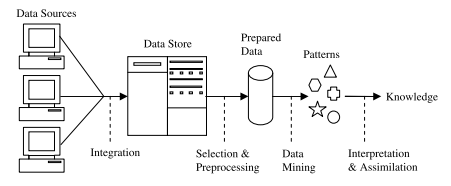
\includegraphics[scale=1.0]{ResearchSteps.png}
		\label{fig:ResearchSteps}
		\caption{A schematic overview how a project involving data mining was done. Multiple data sets were integrated in one database. Feature selection and preprocessing took place to prepare the data. Then the data was mined to find patterns. These patterns were then interpreted and assimilated to discover knowledge on the subject.\cite{bramer2007principles}}
	\end{figure}
	
	% Types of data mining
	Since biomedical data was a wide scope, data mining had several specialisations in different directions. An example would be text data mining, used to find related articles with websites such as Pubmed and Google Scholar. These articles could mention similar genes, diseases or proteins and give additional information about them. Another example would be microarray data mining. This type of data mining focused on extracting entities and pathways that defined a disease or other phenotype. Two other data mining types were proposed. One focused on extracting useful information out of mass spectrometry data points, called proteomic data mining. A second focused more on a molecular level and how these molecules would affect different cell types.\cite{YANG2012S16}
	
	% Reference to earlier made report
	Whichever splits were made in the data mining term for different areas in biomedical data analysis, the techniques were mostly based on statistical analysis and machine learning. A discussion of these two types had been made earlier report\footnote{\label{fn:BDA}Biomedical Data Analysis - \textit{Tim Beishuizen}}.
	
	\subsection{Data Mining Tools}
	\label{subsec:DataMiningTools}
	
	% Introduction data mining tools
	When applying several data mining algorithms to extract results from a data set, a certain tool had to be used that facilitated the use of those algorithms. Several basic tools were available and widely used\footref{fn:BDA}. Since biomedical data had specific characteristics, separate tools or frameworks consisting of those tools were made. These were usually made to create a database with a certain lay-out to put it in or to collect multiple algorithms and alter them specifically for biomedical cases. Many times both were connected as well, for optimized use.
	
	% Data set storage
	To store biomedical data several projects were started. Famous project examples were the Human Genome Project (HGP) that tried to sequence the entire human genome\cite{sawicki1993human} or the Human Connectome Project (HCP) that focused on the brain connectivity.\cite{van2012human} Both consisted of an enormous amount of data that needed to be stored and a tool was created for use in these project, for instance the ConnectomeDB for the HCP.\cite{marcus2011informatics} Similar projects resulted in biomedical databases, such as KEGG\cite{kanehisa2000kegg}, Reactome\cite{joshi2005reactome}, NCBI\cite{edgar2002gene}, GeneCards\cite{safran2010genecards} and HMDB\cite{wishart2007hmdb}. These databases stored data about genes, metabolites and pathways and were used by numerous scientists to completely understand those. More databases were made or are in development, all of them for a specific domain in biomedical research.
	
	% Biomedical data mining frameworks
	Several examples of tools and frameworks of biomedical data mining were available. A framework designed specifically for biomedical data was ImageJ\cite{schindelin2015imagej}. ImageJ could be used for biomedical image analysis and consisted of image processing and analysis techniques. Another example would be Genesis\cite{sturn2002genesis}, a platform for gene expression analysis based on Java and consisting of various preprocessing and clustering algorithms. Similarly the tools GeneCodis3\cite{tabas2012genecodis3}, FatiGO\cite{al2004fatigo} and \cite{zeeberg2003gominer} were created to interpret results from genomics generated data. Similar tools were made for metabolomics, such as Metscape 2\cite{karnovsky2011metscape} and MetaboAnalyst\cite{xia2015metaboanalyst}. The tool G*power3\cite{faul2007g} focused more on statistical analysis of biomedical data.
	
	% Problems data frameworks and databases
	One immediate issue with all of theses existing databases would be that hardly any framework or tool could be found for synchronisation of these databases. Their use was limited to a specific area only without any possibilities to switch in between. An all encompassing framework was not made. Therefore multiple scientists made their work specifically for their specific area. New scientists had a hard time using the newly created tool and tried to create a new one themselves. They would benefit of a new framework that combined aspects of the available tools.\cite{teodoro2009biomedical}
	
	\subsection{Biomedical Knowledge}
	
	% Introduction knowledge
	A last important aspect for data analysis was the available knowledge on the topic. Numerous scientists had done research on various biomedical topics. The knowledge gathered from these topics were available in several different ways.\cite{bellazzi2011data} Usually this information could be found in a textual manner, in books, papers and articles describing the project results. Other information could be found in the earlier mentioned databases, tools and designed algorithms. A third type of knowledge was implicit, skills and information scientists are expected to have or should be trained for if not known with it.\cite{zupan2006knowledge}  All of these were interesting in their own ways.
	
	% Textual knowledge
	Literature knowledge should be the basis for all research. The knowledge found on several different research areas could result in new insights and ideas for unexplored parts. The projects generated this way became knowledge-driven and had hypotheses based on gathered information.\cite{bellazzi2011data} Not only at the start of research projects knowledge was used, as it should be a guide throughout the whole process. In the final project steps their results should be used to improve the existing knowledge, so it could be used in new projects.\cite{zupan2006knowledge}
	
	% Data knowledge
	When looking at projects on implementation level, more interesting data knowledge could be gathered from databases, tools and algorithms. These three could be used to test and answer hypotheses derived from textual knowledge. Mainly these were used for data analysis as known data was gathered from databases, tools were used for their analysis properties and algorithms were implemented, all to improve the project results. When considering data mining and its tools (subsection \ref{subsec:ResearchTarget} and \ref{subsec:DataMiningTools}), everything known plays a big role, too.\cite{bellazzi2011data}
	
	% Scientist knowledge
	A third knowledge type was the implicit knowledge of the scientists conducting a research project. These scientist could have a big difference in background and therefore focus on different goals, tools or algorithms. Scientists should be familiar with using data mining tools to be able to use them, both in a general way as well as for specific tools. Frameworks were made with a certain type of scientist in mind as well, making it important that the desired type of scientist was able to use it, too.\cite{zupan2006knowledge}

	% Problems biomedical knowledge
	These types of knowledge could cause several issues. Projects would not be conducted properly if literature did not back up initial points of view and assumptions. On the other hand data knowledge that stemmed from other research projects could be used for continued improvement in the projects, that could not be done if this type of knowledge was not around. At problems could arise when scientists had different implicit knowledge. A physician at the hospital would not have the same knowledge as a professor in data mining, but would have a better understanding of the usefulness of the results. 
	
	\section{Research Question}
	\label{sec:ResearchQuestion}
	
	% Introduction research question
	The main goal was to create a framework for more efficient data analysis. Based around the four main influencers of data analysis, a main research question was made and divided in five separate sub-questions. The main question would be:\\
	\\
	% Main question
	\emph{What aspects are of importance to include in a framework for Biomedical Engineers to do data analysis more efficient?}\\
	\\
	As discussed earlier the main question could be divided in five different sub-questions. These five sub-questions would have their separate hypothesis. The five questions were:
	
	\begin{enumerate}

	% Data driven question
	\item[\textit{Data driven}] How does the available data influence the choice for a certain data analysis approach?
	
	% Target driven question
	\item[\textit{Target driven}] How does the research goal influence the choice for a certain data analysis approach?
	
	% Data mining tool driven question
	\item[\textit{Tool availability driven}] Which available research tools should be included in this framework?
	
	% Data mining tool extension driven question
	\item[\textit{Tool extension driven}] In which instances is a tool extension required for completion of the framework?
	
	% Data knowledge driven question
	\item[\textit{Knowledge driven}] How must both availability- and lack of knowledge be included in the framework?
	
	\end{enumerate}
	
	\subsection{Data Driven Hypothesis}
	\label{subsec:DataDrivenHypothesis}
	
	% Data challenges hypotheses
	A major part in a data driven analysis approach was the presence of challenges with preprocessing the data. Data volume, dimensionality, complexity, heterogeneity and quality challenges all were issues to be tackled, some of them more interesting than others. The most approachable three challenges would be the data volume, dimensionality and quality challenges. These three problems were well known defined problems with various ways to deal with them, however no perfect answer existed yet. Data dimensionality could be tackled by various feature selection and reduction algorithms, such as principal component analysis, significance testing and clustering. Low data volume could be tackled by various data generation algorithms based on nearest neighbours and interpolation. At last data quality can be improved by handling for example missing values with interpolation and outliers with outlier detection.
	
	\subsection{Target Driven Hypothesis}
	\label{subsec:TargetDrivenHypothesis}
	
	% Target driven hypothesis, step one
	To reach a certain goal, several steps have to be taken. While the steps could be vastly different, it rarely would not start with a global analysis to localize possible issues and interesting features in the data. A statistical analysis should be very beneficial for doing such a global analysis and a possibility for adding that to the framework would be a great benefit.
	
	% Several algorithms for the goal
	Other steps were less clear. Follow-up steps after a global data analysis would be to try out several basic techniques known to achieve that goal. After computing the results, they could be used to revise the technique for better results or disregard it completely. This more specific data mining step would include trying out several machine learning techniques or better feature selection.
	
	% Specific algorithms for the goal
	The final steps to achieve the goal would be very personalized for every project. To approach these final steps numerous things should be considered and done already in previous steps. This would mean that the scientist itself would have the best idea how to achieve that goal with the knowledge gathered from the first couple of steps. Therefore it would not be useful to guide someone in this part of the data analysis.
		
	\subsection{Tool Availability Driven Hypothesis}
	\label{subsec:ToolAvailabilityDrivenHypothesis}
	
	% Introduction tool availability Python, scipy, scikit-learn, TPOT
	Tools to be included in the final framework should be focused around the data driven and target driven desired techniques. This would mean that it should include tools for feature reduction and selection, data generation, missing value and outlier handling, global analysis and machine learning. On top of that the tools should be able to communicate easily, as they might be used in sequence.
	
	% Scikit-learn, TPOT
	The package scikit-learn from python provided already several algorithms for this problem and would be a good start for the framework. Several feature selection and machine learning algorithms were present and easily useable. A very welcome addition to scikit-learn was Tree-based Pipeline Optimization Tool (TPOT) that made finding the best machine learning algorithm with the best hyperparameters automated. TPOT used both algorithms from scikit-learn and algorithms made by the user. These two would be good tools for a successful data mining project.
	
	% Scipy, Python, Anaconda
	Both scikit-learn and TPOT were packages for Python. Another Python package that would be helpful for the project would be the SciPy package. SciPy was very useful for statistical analysis, due to the broad level of available statistical algorithms in it. Those algorithms would be good for global analysis and outlier detection as well as possible feature reduction. Anaconda was a Python distribution that could help you automatically download multiple packages, among others scikit-learn, SciPy and the widely used NumPy. This Anaconda would therefore be a welcome addition, too.
	
	\subsection{Tool Extension Driven Hypothesis}
	\label{subsec:ToolExtensionDrivenHypothesis}
	
	% Initroduction tool extension
	With the mention of Scikit-learn, TPOT and SciPy, most aspects desired in the framework were at least partly covered. These three most likely were not perfect for every data set though and might need more programming to better suit the framework. Also several data driven preprocessing algorithms to TPOT would be helpful, making TPOT more suitable for biomedical data. 
	
	% Volume generation & missing value handling
	With the mentioned tools a good base for most of the desired parts in the framework were mentioned. The only two aspects that were not discussed, yet, would be the volume generation and missing value handling. Both of these and possible more algorithms for the other aspects could be programmed to show more variety in preprocessing and data mining.
	
	% Initial statistical analysis tool
	Some statistical methods were available for analysis in SciPy. These statistical methods still had to be called for privately for SciPy and no selection was made for an initial global analysis. Therefore a new method for doing that global analysis should be made, that borrowed methods from SciPy to give the use insight in the dataset. This would mean it needed basic statistical methods, such as descriptive statistics computation, significance testing and multicollinearity testing. 
	
	% Database integration
	At last numerous online databases were available with both genomic and metabolic data in them, such as NCBI and KEGG. Some people made some possible integration packages for these databases, however these were not widely known or used. A possible tool extension for the framework would be a possibility to download specific parts of these databases that would contain useful information, so these can be used for further investigation of the genomic or metabolic data.
	
	\subsection{Knowledge Driven Hypothesis}
	\label{subsec:KnowledgeDrivenHypothesis}
	
	% Created for biomedical engineering students
	The framework would be mainly created for the cBio group. Since this group mainly consisted of either experienced employees that were already doing a research projects or less experienced students, the best focus for this framework would be biomedical students. They would benefit the most for such a framework that could help them at the start of their projects. The scope of the framework would then be people that had some minor programming skills and would need guidance for better understanding and efficiency.
	
	% Create a GUI
	Since inexperienced programmers would not know immediately how to program in possibly a different language, a graphical user interface (GUI) could be of help as well. This GUI could help mainly in the global analysis, but maybe also in running some initial calculations with TPOT. When using this GUI, programming would be less important as a skill and therefore people would not need to figure out how the framework was designed. For programmers that needed to use more specific methods, it would still be possible to use it as packages for their own project.
	
	% Create a user manual with also examples how to use everything
	To understand everything without too much difficulty a user manual should be made. This user manual should include (publicly available) data sets and show how the framework should be used exemplary with these data sets. This manual and explanations would make the framework more accessible for both inexperienced and experienced programmers and would help them understand it quicker.
	
	\bibliography{../References/Citings} 
	\bibliographystyle{ieeetr}
	
	\appendix
	
\end{document}
